%%%%%%%%%%%%%%%%%%%%%%%%%%%%%%%%%%%%%%%%%
% Beamer Presentation
% LaTeX Template
% Version 1.0 (10/11/12)
%
% This template has been downloaded from:
% http://www.LaTeXTemplates.com
%
% License:
% CC BY-NC-SA 3.0 (http://creativecommons.org/licenses/by-nc-sa/3.0/)
%
%%%%%%%%%%%%%%%%%%%%%%%%%%%%%%%%%%%%%%%%%

%----------------------------------------------------------------------------------------
%	PACKAGES AND THEMES
%----------------------------------------------------------------------------------------

\documentclass{beamer}

\mode<presentation> {

% The Beamer class comes with a number of default slide themes
% which change the colors and layouts of slides. Below this is a list
% of all the themes, uncomment each in turn to see what they look like.

%\usetheme{default}
%\usetheme{AnnArbor}
%\usetheme{Antibes}
%\usetheme{Bergen}
%\usetheme{Berkeley}
%\usetheme{Berlin}
%\usetheme{Boadilla}
%\usetheme{CambridgeUS}
%\usetheme{Copenhagen}
%\usetheme{Darmstadt}
%\usetheme{Dresden}
%\usetheme{Frankfurt}
%\usetheme{Goettingen}
%\usetheme{Hannover}
%\usetheme{Ilmenau}
%\usetheme{JuanLesPins}
%\usetheme{Luebeck}
\usetheme{Madrid}
%\usetheme{Malmoe}
%\usetheme{Marburg}
%\usetheme{Montpellier}
%\usetheme{PaloAlto}
%\usetheme{Pittsburgh}
%\usetheme{Rochester}
%\usetheme{Singapore}
%\usetheme{Szeged}
%\usetheme{Warsaw}

% As well as themes, the Beamer class has a number of color themes
% for any slide theme. Uncomment each of these in turn to see how it
% changes the colors of your current slide theme.

%\usecolortheme{albatross}
%\usecolortheme{beaver}
%\usecolortheme{beetle}
%\usecolortheme{crane}
%\usecolortheme{dolphin}
%\usecolortheme{dove}
%\usecolortheme{fly}
%\usecolortheme{lily}
%\usecolortheme{orchid}
%\usecolortheme{rose}
%\usecolortheme{seagull}
%\usecolortheme{seahorse}
%\usecolortheme{whale}
%\usecolortheme{wolverine}

%\setbeamertemplate{footline} % To remove the footer line in all slides uncomment this line
%\setbeamertemplate{footline}[page number] % To replace the footer line in all slides with a simple slide count uncomment this line

%\setbeamertemplate{navigation symbols}{} % To remove the navigation symbols from the bottom of all slides uncomment this line
}
\usepackage{amsthm,amsmath,amssymb,upgreek,marvosym,mathtools}
\usepackage{graphicx}
\graphicspath{ {./pics/} }

\usepackage{booktabs} % Allows the use of \toprule, \midrule and \bottomrule in tables
\usepackage{xcolor}
\usepackage{fancyvrb}
\usepackage{float}
\usepackage{pgffor}% http://ctan.org/pkg/pgffor
\usepackage{pdfpages}
\usepackage{pifont}% http://ctan.org/pkg/pifont
\usepackage{subfig}
%\newtheorem{lemma}{Lemma}
\newtheorem{reduction}{Reduction}
\newtheorem{proposition}{Proposition}
\newtheorem{claim}{Claim}
\newtheorem{scolium}{Scolium}   %% And a not so common one.
%\newtheorem{definition}{Definition}
\newtheorem{construction}{Construction}

\usepackage{tkz-graph}
\usepackage{arydshln}
\usepackage{comment}
\setbeamertemplate{enumerate items}[default]
\usetikzlibrary{automata, positioning,arrows,shapes,decorations.pathmorphing}
\newcommand{\distras}[1]{%
  \savebox{\mybox}{\hbox{\kern3pt$\scriptstyle#1$\kern3pt}}%
  \savebox{\mysim}{\hbox{$\sim$}}%
  \mathbin{\overset{#1}{\kern\z@\resizebox{\wd\mybox}{\ht\mysim}{$\sim$}}}%
}
 \tikzset{
node distance=3cm, % specifies the minimum distance between two nodes. Change if necessary.
every state/.style={thick, fill=gray!10}, % sets the properties for each ’state’ node
initial text=$ $, % sets the text that appears on the start arrow
}

\newcommand{\db}{$\mathbf{db}$}
\newcommand{\sjfq}{\texttt{sjfCQA}}
\newcommand{\bcq}{\texttt{bcq}}
\newcommand{\prob}[1]{\textsc{certainty}($#1$)}
\newcommand{\fo}{$\mathbf{FO}$}
\newcommand{\p}{$\mathbf{P}$}
\newcommand{\lspace}{$\mathbf{L}$}
\newcommand{\coNP}{$\mathbf{coNP}$}
\newcommand{\und}[1]{\underline{#1}}
\newcommand{\nl}{$\mathbf{NL}$}


\title[LIP with limited memory]{Accelerating Joins with Filters: Keeping a Limited Memory is Robust} % The short title appears at the bottom of every slide, the full title is only on the title page

\author{Nicholas Corrado \and Xiating Ouyang} % Your name
\institute[] % Your institution as it will appear on the bottom of every slide, may be shorthand to save space
{
University of Wisconsin-Madison \\ % Your institution for the title page
\medskip
\textit{} % Your email address
}
\date{} % Date, can be changed to a custom date




\begin{document}

\begin{frame}
\titlepage % Print the title page as the first slide
\end{frame}


\begin{frame}
\frametitle{Star Schema}
\begin{figure}
  \centering
  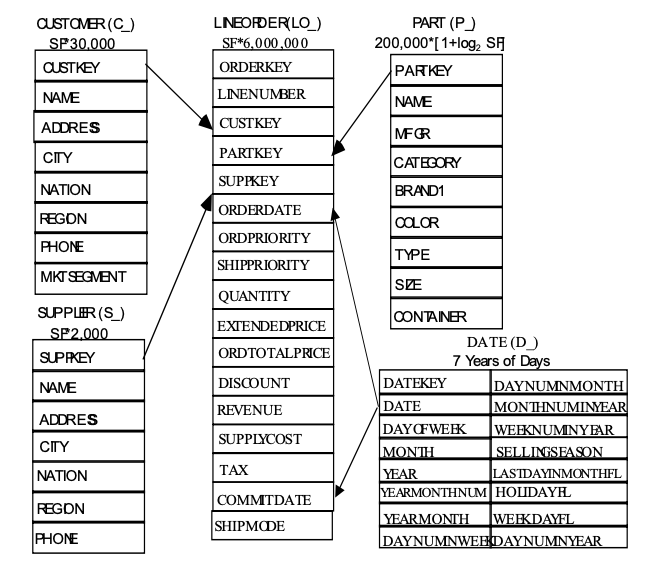
\includegraphics[height=0.7\textheight,keepaspectratio]{star-schema}
\end{figure}

\begin{itemize}
  \item Gigantic intermediate tables
  \item Filtering ahead of time before join
\end{itemize}
\end{frame}

% lip slides here



\foreach \n in {1,...,25} {%
  \begin{frame}[noframenumbering]
  \frametitle{Lookahead Information Passing (LIP)}
  \begin{figure}
    \centering
    \includegraphics[page={\n},height=0.7\textheight,keepaspectratio]{lip-animation}
    \end{figure}
  \end{frame}
}


\begin{frame}[noframenumbering]
  \frametitle{Lookahead Information Passing (LIP)}
  \begin{figure}
    \centering
    \includegraphics[page={26},height=0.7\textheight,keepaspectratio]{lip-animation}
  \end{figure}
  \pause
  \begin{itemize}
    \item Using statistics from all previous batches
    \item Just the previous $k$ \pause --- LIP-$k$
  \end{itemize}
\end{frame}
% lip slides above

\begin{frame}
  \frametitle{Implementation and benchmarking}
  \begin{figure}
    \centering
    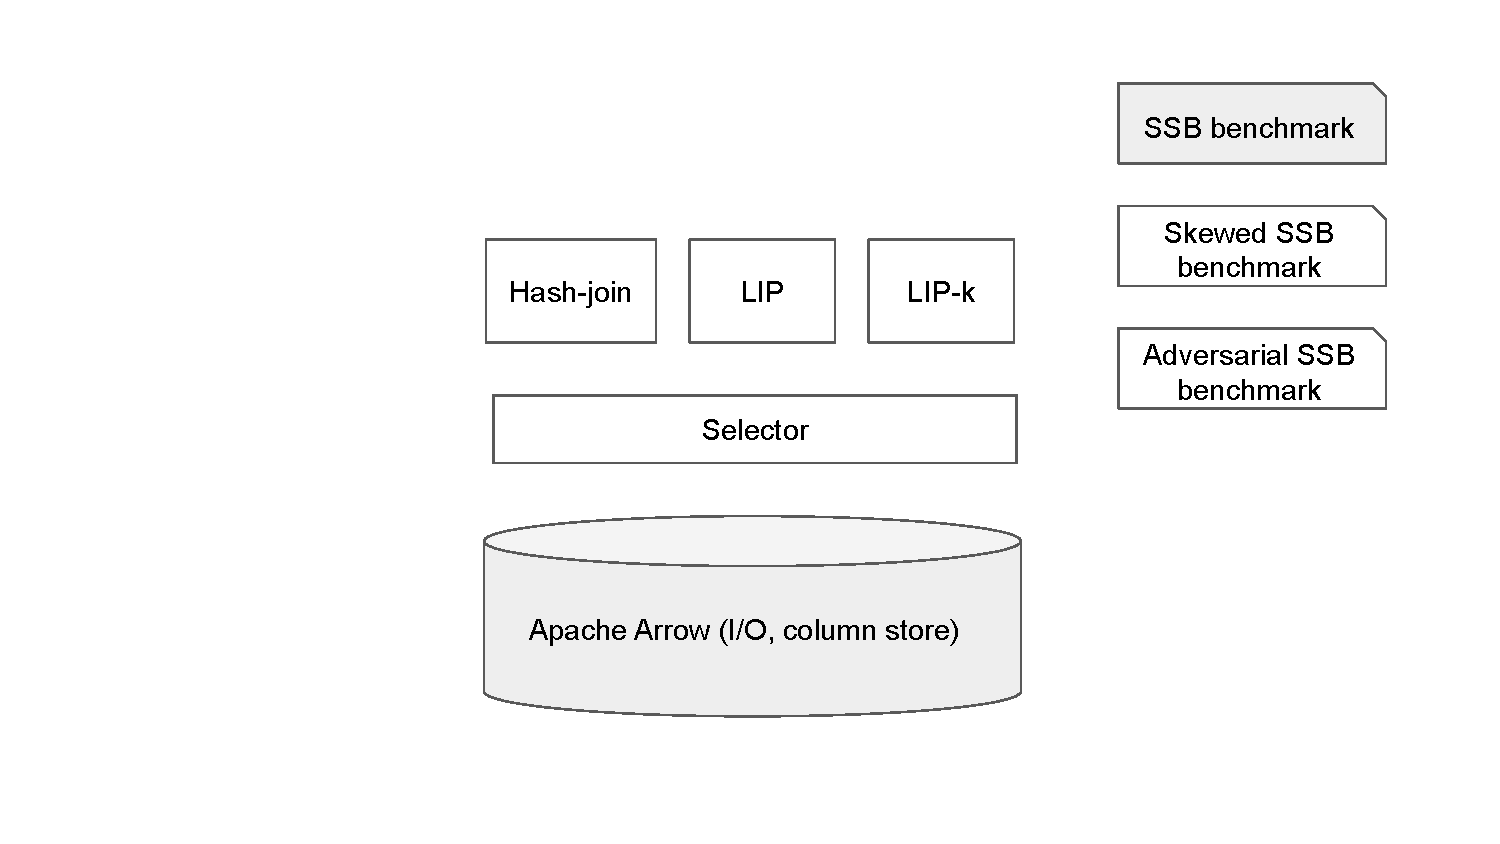
\includegraphics[height=0.7\textheight,keepaspectratio]{implementation}
  \end{figure}
\end{frame}


\begin{frame}
  \frametitle{Experiments}
  \begin{figure}
    \centering
    %\includegraphics[height=0.7\textheight,keepaspectratio]{time-graph}
  \end{figure}
\end{frame}



\begin{frame}
\frametitle{LIP is solving an online problem}
\begin{itemize}
  \item Tuples arriving one at a time
  \item Upon arrival, decide a sequence of filters
  \item Minimize the total probes
  \item Deterministic! \pause
\end{itemize}

\begin{theorem}
  Let $n$ be the number of filters in the LIP problem. There is no deterministic mechanism $\mathcal{M}$ achieving a competitive ratio less than $n$ for the \textsc{LIP} problem.
\end{theorem}

\pause
\begin{itemize}
  \item Not observed in practice, but a theoretical lower bound
  \item Randomness?
\end{itemize}

\end{frame}



\begin{frame}
  \frametitle{Competitive ratio vs.\ $k$ on Uniform}
  \begin{figure}
    \centering
    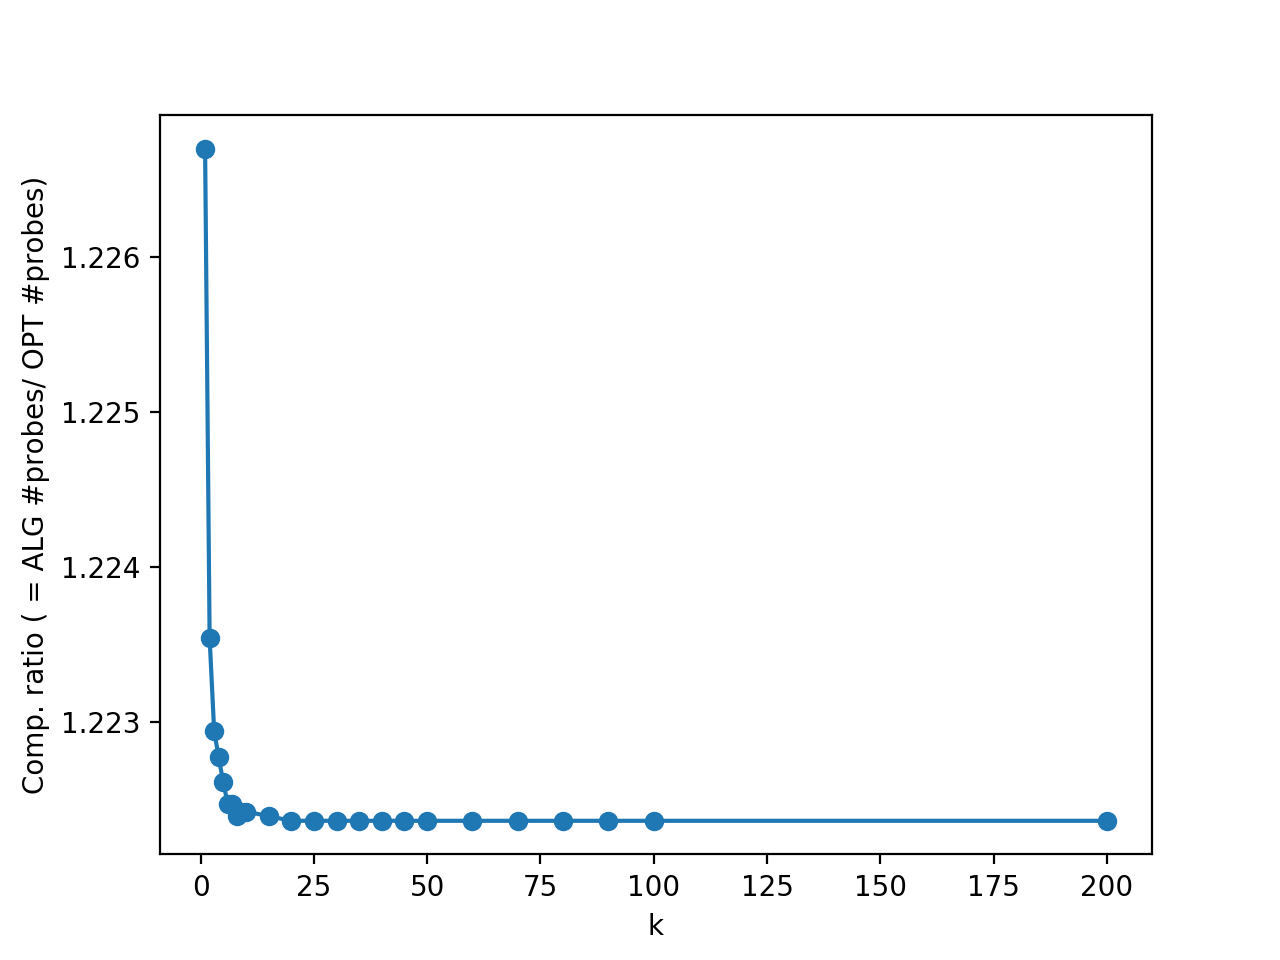
\includegraphics[height=0.7\textheight,keepaspectratio]{cr-k-uniform}
  \end{figure}
\end{frame}



\begin{frame}
  \frametitle{Competitive ratio vs.\ $k$ on Adversarial}
  \begin{figure}
    \centering
    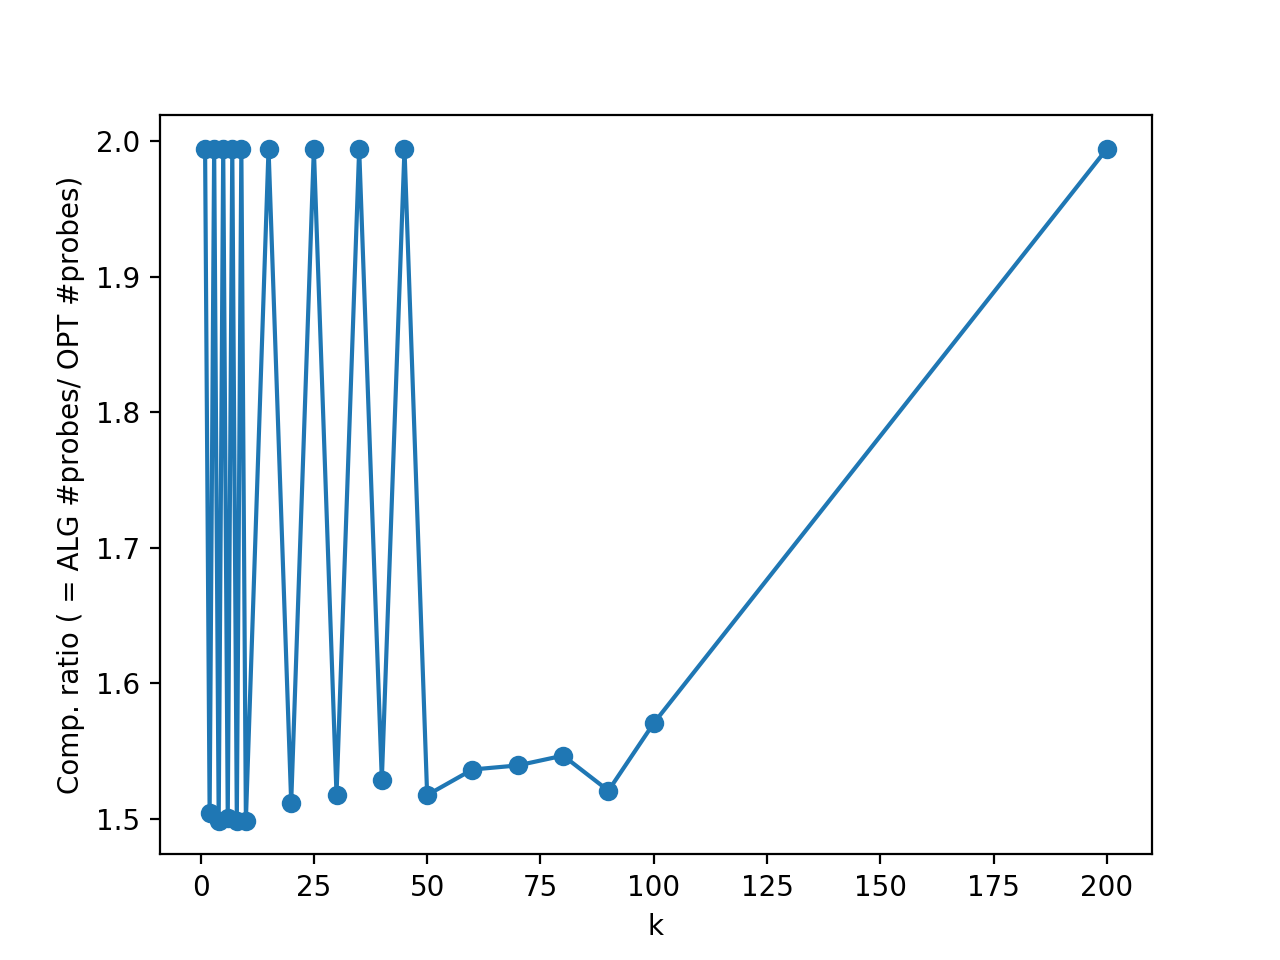
\includegraphics[height=0.7\textheight,keepaspectratio]{cr-k-skewed}
  \end{figure}
\end{frame}



\begin{frame}
\frametitle{Conclusion}

  \begin{itemize}
    \item Implemented LIP and its variant LIP-$k$
    \item LIP-$k$ is better than LIP in the adversarial/skewed settings
    \item Randomness to achieve better robustness guarantee
  \end{itemize}
\end{frame}


\begin{frame}
\Huge{Thank you!}
\end{frame}

\begin{frame}
\Huge{Questions?}
\end{frame}
%----------------------------------------------------------------------------------------

\end{document}
